%!TEX root = ../dissertation.tex
\chapter{Future Direction of Research}
\label{chap:Future}
\section{Biomechanics Applications: Articular Cartilage}
Osteoarthritis (OA), the breakdown of the articular cartilage, affects the lives of million adults. Although there are treatments to manage the condition, there is no cure nor any completely effective method of preventing the disease. As such, it is essential to comprehensively study factors that contribute to OA in order to guide the development of improved treatments. Research in this field has the potential to substantially improve our understanding of multi-scale articular cartilage mechanics, which assists efforts to investigate degenerative pathways. The focus of this direction of the future research is  on the modeling and simulation of the micro-structure of the articular cartilage, given that it is comprised of both a fluid phase (water and electrolytes) and a solid phase (collagen fibrils, proteoglycans, and chondrocytes). Figure~\ref{fig:AC} demonstrates the proposed FSI modeling strategy. 
\begin{figure}
	\centering
	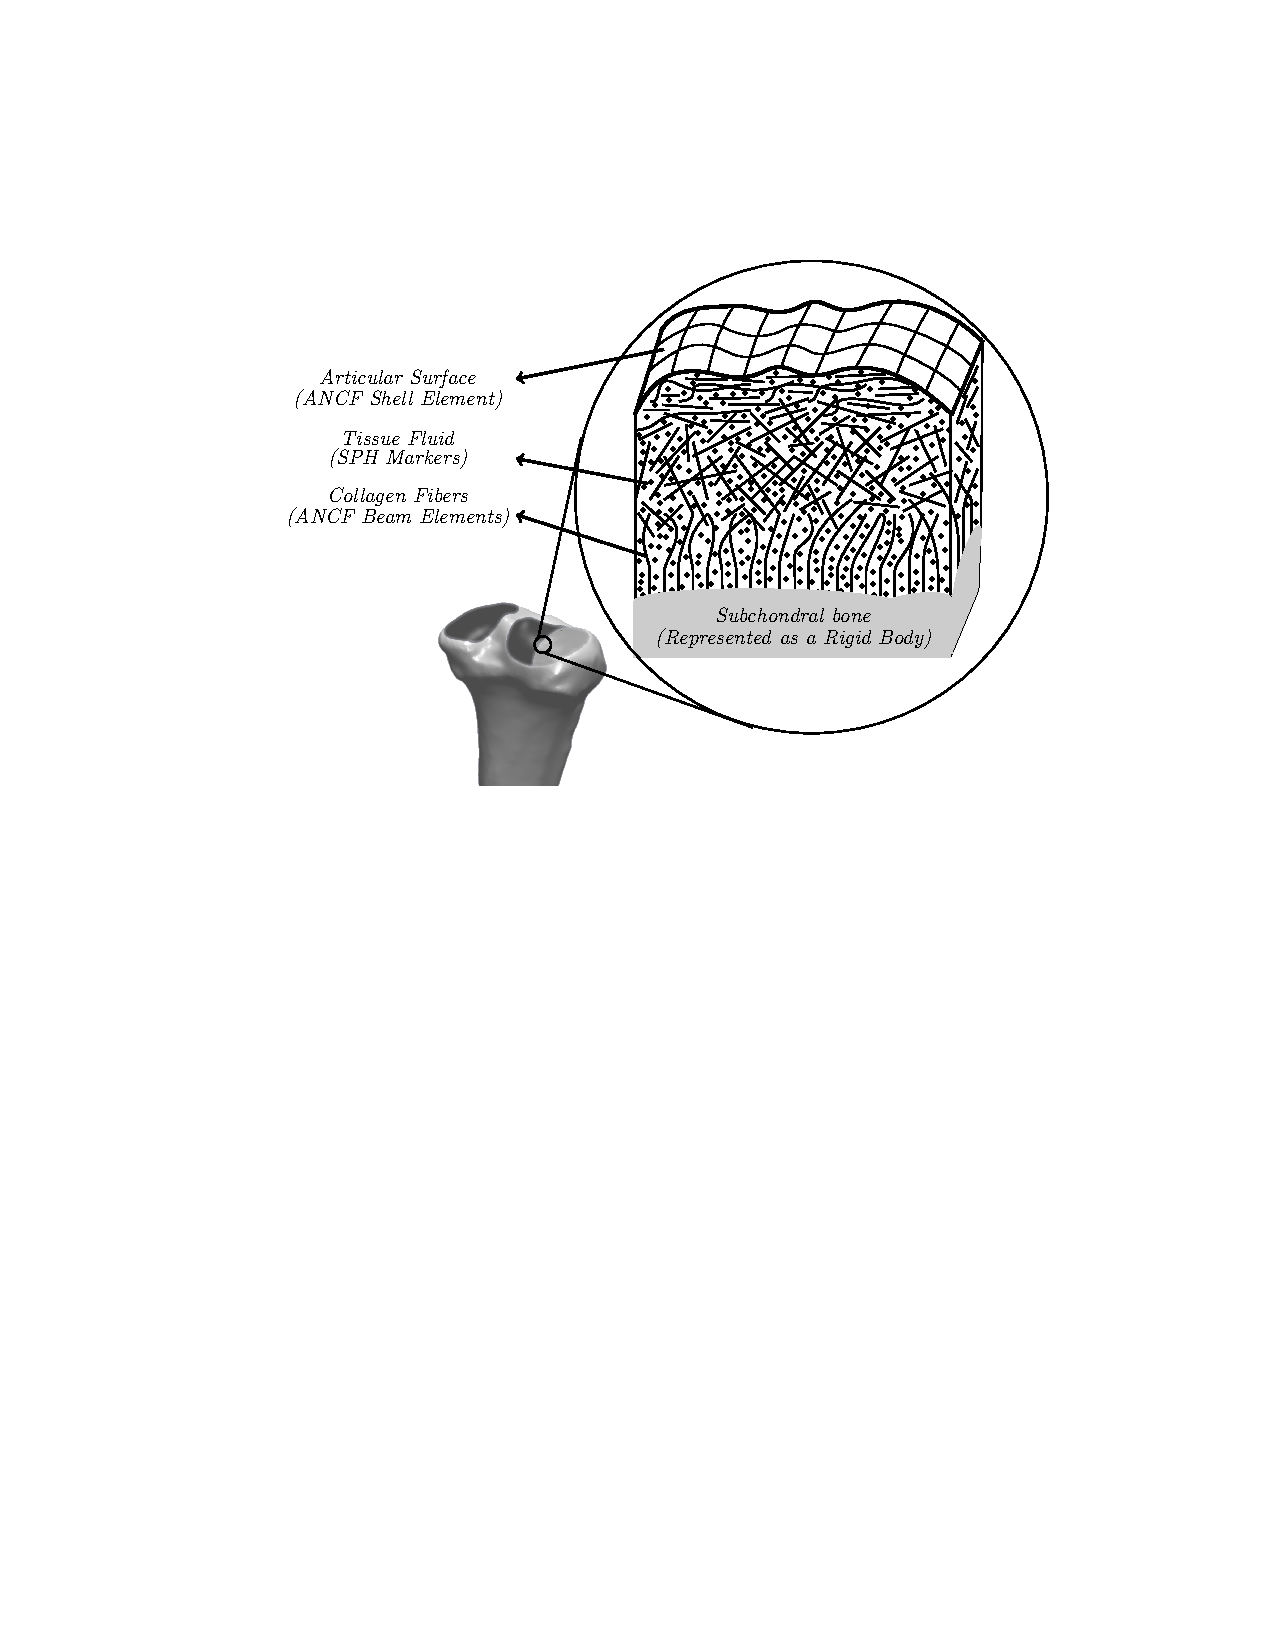
\includegraphics[width=10cm]{images/AC.pdf}
	\captionof{figure}{Fluid-solid interaction modeling strategy of the articular cartilage}
	\label{fig:AC}
\end{figure}
 Preliminary results of the small-scale FSI model are demonstrated in Figure~\ref{fig:IR}.
\begin{figure}
	\centering
	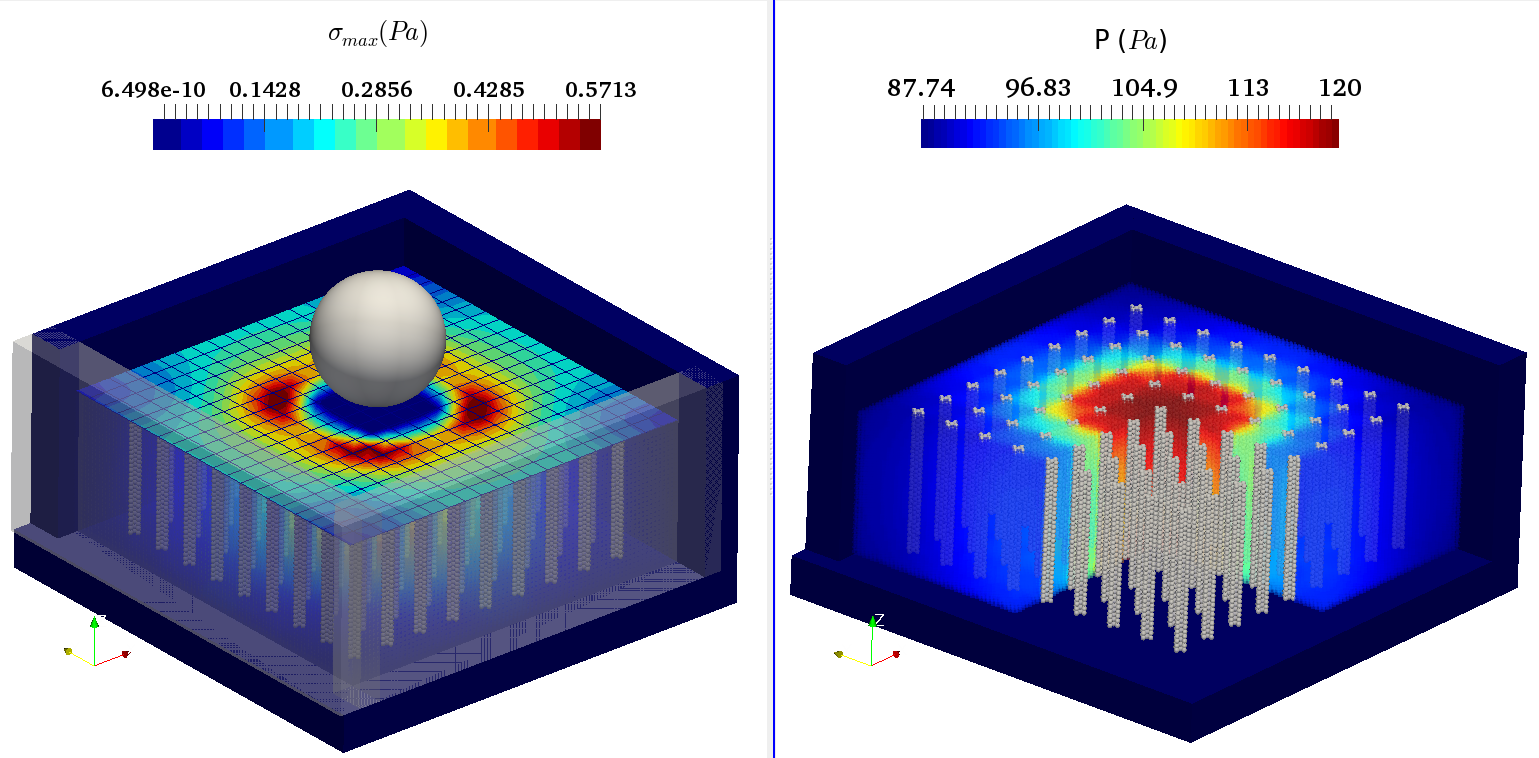
\includegraphics[width=0.7\linewidth]{images/fibers.png}
	\captionof{figure}{Preliminary results of the articular cartilage FSI model. Displacement and stress field on the articular surface (top and bottom left, respectively). Pressure and velocity distribution inside the interstitial fluid (top and bottom right, respectively)}
	\label{fig:IR}
\end{figure}
\section{Data Driven CFD}
\section{Hybrid Eulerian-Lagrangian Discretization : MPM}
\section{Higher-order Lagrangian Discretization : GMLS}